\chapter{Desarrollo}
\section{Análisis de viabilidad y factibilidad}
En esta sección, se presenta el análisis de viabilidad y factibilidad del prototipo de aplicación móvil de apoyo para la traducción de español a Lengua de Señas Mexicana (LSM) empleando técnicas de Procesamiento de Lenguaje Natural (PLN) y modelado 3D, con el objetivo de evaluar si existen las condiciones técnicas, humanas, tecnológicas y financieras necesarias para su desarrollo exitoso del mismo. En primer lugar, se analiza la viabilidad, considerando los conocimientos del equipo, las tecnologías disponibles, las condiciones de ejecución y el potencial de escalabilidad del prototipo. Posteriormente, se estudia la factibilidad, enfocándose en los recursos financieros, humanos y tecnológicos, así como en el tiempo estimado para completar el proyecto.\\

\subsection{Viabilidad}
El análisis de viabilidad considera los conocimientos técnicos del equipo, la madurez de las tecnologías disponibles y las condiciones actuales para el desarrollo. Este análisis permite evaluar si el proyecto puede llevarse a cabo de manera exitosa bajo las condiciones planteadas.

\subsubsection{Conocimientos y experiencia}
El equipo de desarrollo posee conocimientos en Procesamiento de Lenguaje Natural (PLN), así como habilidades básicas en animaciones y recursos visuales. Aunque la experiencia en animación 3D orientada a señas, en programación de aplicaciones móviles y en el manejo de la Lengua de Señas Mexicana (LSM) es limitada, se considera factible adquirir y aplicar los conocimientos necesarios mediante el uso de recursos de investigación, bibliotecas especializadas y la colaboración con expertos en LSM, tomando en cuenta la versión correspondiente al uso y documentación del año 2024. Esta disposición de aprendizaje y fortalecimiento de competencias respalda la viabilidad técnica del proyecto en función de las capacidades del equipo.

De manera complementaria, se cuenta con diversas tecnologías que facilitarán la implementación del prototipo, tal como se describe a continuación.

\subsubsection{Tecnologías disponibles}
Actualmente, existen diversas tecnologías y herramientas que facilitan la creación de sistemas de traducción de texto a señas, tales como conjunto de datos de señas en video, motores de animación 3D y frameworks para el desarrollo de aplicaciones móviles. Asimismo, se dispone de plataformas de código abierto que permiten representar señas mediante modelos animados o videos precargados, optimizando así los recursos disponibles para el desarrollo de prototipos.

Las tecnologías consideradas para el presente proyecto incluyen:
\begin{itemize} 
	\item Librerías y conjunto de datos de señas mexicanas (videos de señas). 
	\item Herramientas de animación 3D como Blender (versión 4.4.3) o Unity (versión 6.1), así como motores ligeros compatibles con aplicaciones móviles. 
	\item Frameworks de desarrollo móvil como Flutter (versión 3.29.3) y React Native (versión 0.79). 
	\item Herramientas de Procesamiento de Lenguaje Natural (PLN) para el análisis y segmentación de frases en español. 
\end{itemize}

\subsubsection{Condiciones para la ejecución}
El proyecto se desarrolla en el marco de un trabajo terminal académico, lo que garantiza el acceso a recursos institucionales, asesoría especializada y bibliografía técnica actualizada. De igual manera, el creciente interés social y académico por fomentar la inclusión de la comunidad sorda en México genera un entorno favorable para la implementación de este tipo de iniciativas, fortaleciendo así las condiciones de ejecución del prototipo.

Además de considerar las condiciones actuales para la ejecución del proyecto, se ha previsto su potencial de crecimiento a futuro, como se expone a continuación.

\subsubsection{Escalabilidad}
Aunque el proyecto está concebido inicialmente como un prototipo académico, su arquitectura modular permitirá una potencial expansión hacia una versión comercial en etapas futuras. Esta expansión contemplaría la incorporación de un mayor número de frases, la optimización de los motores de animación y la adaptación a múltiples dispositivos o plataformas. No obstante, se reconoce que dicho crecimiento requerirá una inversión adicional en recursos financieros y humanos, factores que deberán evaluarse conforme avance el desarrollo del proyecto.

\subsection{Factibilidad}
La factibilidad del proyecto se analiza considerando los recursos financieros, humanos y tecnológicos disponibles, así como el tiempo estimado para su desarrollo y finalización.

\subsubsection{Recursos financieros}
El presente apartado tiene como objetivo evaluar los costos asociados al desarrollo, despliegue y potencial comercialización del prototipo. 

Para ello, se plantea un análisis financiero estructurado en dos niveles: 

\begin{itemize}
	\item \textbf{Enfoque académico:} Incluye estimaciones de costos simbólicos aproximados del mercado laboral en México correspondientes al año 2025 [CITA IEEE], considerando el uso de recursos propios, herramientas gratuitas y asesorías puntuales. Este enfoque representa fielmente la ejecución del proyecto dentro de un marco académico.
	
	\item \textbf{Enfoque exploratorio de comercialización:} Presenta una simulación de costos reales basada en tarifas aproximadas de mercado laboral en México correspondientes al año 2025 [CITA IEEE], incluyendo sueldos profesionales, licencias, infraestructura tecnológica y servicios externos. Este análisis permite anticipar los requerimientos financieros de una futura etapa de comercialización.
\end{itemize}

Ambas perspectivas se estructuran mediante dos métodos complementarios de análisis financiero:

\begin{itemize}
	\item \textbf{Estimación por recursos:} Identifica y valora los insumos materiales, humanos y tecnológicos necesarios para el desarrollo y operación del prototipo.
	\item \textbf{Estimación por actividades:} Desglosa las tareas específicas del proyecto, asignando tiempos estimados y costos unitarios para cada una.
\end{itemize}

Esta estructura metodológica permite identificar con precisión los recursos involucrados, calcular el presupuesto total estimado y analizar la factibilidad financiera del proyecto, tanto en su ejecución académica como en un escenario de comercialización futuro.

\paragraph{\textbf{Informe de costos de creación del prototipo.}} 
Este informe presenta el análisis financiero asociado al desarrollo y creación del prototipo de la aplicación móvil de apoyo para la traducción de frases del español a la Lengua de Señas Mexicana (LSM) mediante Procesamiento de Lenguaje Natural (PLN) y modelado 3D. El objetivo es identificar y estructurar los costos necesarios para garantizar la factibilidad del proyecto en su etapa de creación.

\paragraph{\textbf{Presupuesto mediante recursos.}} 
Dentro del análisis basado en recursos, el proceso de desarrollo se ha estructurado en tres etapas principales, cada una integrada por actividades específicas que permiten avanzar de manera ordenada, asegurando la calidad y funcionalidad del prototipo final. Las etapas contempladas son:

\begin{itemize}
	\item \textbf{Creación del prototipo}. 
	\item \textbf{Despliegue del prototipo}.
	\item \textbf{Evaluación financiera}. 
\end{itemize}

Cada una de estas etapas será detallada en los apartados siguientes.

\paragraph{\textbf{Creación del prototipo.}} 
Esta primera etapa abarca todas las actividades necesarias para el desarrollo inicial del prototipo: definición de objetivos, especificaciones técnicas, requisitos, diseño de animaciones, etc. Aquí se implementan técnicas de PLN para la segmentación de frases y modelado/animación 3D para representar las señas en LSM.

\paragraph{\textbf{Despliegue del prototipo.}} 
Incluye acciones para poner en funcionamiento la app en Android (versión 14), publicación, configuración técnica, documentación técnica y pruebas piloto con usuarios. Esta retroalimentación permitirá ajustar y mejorar la experiencia de uso.

\paragraph{\textbf{Evaluación financiera.}} 
Implica analizar los costos de las etapas anteriores y valorar beneficios esperados como impacto social, accesibilidad y sostenibilidad. Aunque el proyecto tiene fines académicos, se incluye un análisis básico de posibilidad de escalamiento.

Este enfoque estructurado de desarrollo permite garantizar una planeación clara y eficiente, considerando los elementos técnicos, operativos y financieros necesarios para la ejecución del proyecto.

Por último, como medida preventiva ante posibles riesgos o imprevistos, se contempla una reserva de contingencia equivalente al 15\% del costo total estimado.


\paragraph{\textbf{Análisis de recursos.}} 
\paragraph{\textbf{Costos de servicios.}} 
A continuación, se detallan los costos asociados a los servicios necesarios para el desarrollo del prototipo, considerando un periodo estimado de ejecución de cuatro meses. Se incluyen los servicios con ambos enfoques, el académico y el exploratorio de comercialización.


\begin{table}[H]
	\centering
	\renewcommand{\arraystretch}{1.5}
	\setlength{\tabcolsep}{12pt}
	\resizebox{\textwidth}{!}{%
		\begin{tabular}{|l|r|r|r|}
			\hline
			\textbf{Recurso} & \textbf{Costo mensual (MXN \$)} & \textbf{Costo a 4 meses (MXN \$)} & \textbf{Costo a 1 año (MXN \$)} \\ \hline
			Electricidad e Internet (compartido entre integrantes) & \$500.00 & \$2,000.00 & \$6,000.00 \\ \hline
			Almacenamiento en la nube (Google Drive / GitHub) & \$300.00 & \$1,200.00 & \$3,600.00 \\ \hline
			Pruebas en dispositivos Android (emulador físico o virtual) & \$500.00 & \$2,000.00 & \$6,000.00 \\ \hline
			Reserva para servicios externos o pruebas adicionales & \$1,000.00 & \$4,000.00 & \$12,000.00 \\ \hline
			\textbf{Total estimado de servicios} & \textbf{\$2,300.00} & \textbf{\$9,200.00} & \textbf{\$27,600.00} \\ \hline
		\end{tabular}%
	}
	\caption{Costos estimados de servicios en el escenario académico durante la creación del prototipo.}
	\label{tab:costos_servicios}
\end{table}

\begin{table}[H]
	\centering
	\renewcommand{\arraystretch}{1.5}
	\setlength{\tabcolsep}{10pt}
	\resizebox{\textwidth}{!}{%
		\begin{tabular}{|l|r|r|r|}
			\hline
			\textbf{Recurso o servicio} & \textbf{Costo mensual (MXN \$)} & \textbf{Costo a 4 meses (MXN \$)} & \textbf{Costo a 1 año (MXN \$)} \\ \hline
			Electricidad e internet (oficina dedicada) & \$2,500.00 & \$10,000.00 & \$30,000.00 \\ \hline
			Renta de espacio de coworking (para 3 personas) & \$9,000.00 & \$36,000.00 & \$108,000.00 \\ \hline
			Suscripción a plataformas de desarrollo (GitHub Copilot, Blender Studio, etc.) & \$800.00 & \$3,200.00 & \$9,600.00 \\ \hline
			API de lenguaje natural (OpenAI GPT, DialogFlow) & \$1,000.00 & \$4,000.00 & \$12,000.00 \\ \hline
			Servicios de almacenamiento en la nube (Google Cloud, Firebase, etc.) & \$750.00 & \$3,000.00 & \$9,000.00 \\ \hline
			Servidor para aplicación móvil (Firebase/AWS) & \$1,200.00 & \$4,800.00 & \$14,400.00 \\ \hline
			Licencia de software para animación (Unity, MediaPipe, etc.) & \$1,500.00 & \$6,000.00 & \$18,000.00 \\ \hline
			Validación profesional de señas LSM (freelancer mensual) & \$5,000.00 & \$20,000.00 & \$60,000.00 \\ \hline
			Servicios de soporte técnico y mantenimiento & \$3,000.00 & \$12,000.00 & \$36,000.00 \\ \hline
			Marketing digital (redes sociales, web, SEO) & \$2,000.00 & \$8,000.00 & \$24,000.00 \\ \hline
			Traducción y adaptación de contenido LSM (consultoría externa) & \$4,000.00 & \$16,000.00 & \$48,000.00 \\ \hline
			\textbf{TOTAL ESTIMADO} & \textbf{\$30,750.00} & \textbf{\$123,000.00} & \textbf{\$369,000.00} \\ \hline
		\end{tabular}%
	}
	\caption{Costos estimados de servicios en un escenario comercial para la creación del prototipo.}
	\label{tab:costos_comercial}
\end{table}

\paragraph{\textbf{Compras no recurrentes.}} 
En esta sección se presentan los costos estimados de artículos y adquisiciones necesarias para la creación del prototipo, clasificadas como compras no recurrentes. Estas compras representan inversiones únicas que no implican costos periódicos, pero que son fundamentales para el correcto desarrollo y prueba de la aplicación.

\begin{table}[H]
	\centering
	\renewcommand{\arraystretch}{1.5}
	\setlength{\tabcolsep}{8pt}
	\resizebox{\textwidth}{!}{%
		\begin{tabular}{|l|c|r|r|}
			\hline
			\textbf{Recurso} & \textbf{Unidades} & \textbf{Costo unitario (MXN \$)} & \textbf{Costo total (MXN \$)} \\ \hline
			Equipo de cómputo personal (propio de los integrantes) & 3 & -- & -- \\ \hline
			Dispositivo Android para pruebas físicas & 1 & -- & -- \\ \hline
			Capacitación online (cursos: Blender, MediaPipe, PLN) & 3 cursos & \$800.00 & \$2,400.00 \\ \hline
			Compra de modelos 3D o recursos gráficos (opcional) & 1 paquete & \$2,500.00 & \$2,500.00 \\ \hline
			\textbf{Total compras no recurrentes} & & & \textbf{\$4,900.00} \\ \hline
		\end{tabular}%
	}
	\caption{Costos estimados de artículos y compras no recurrentes en el escenario académico.}
	\label{tab:compras_no_recurrentes}
\end{table}

\noindent \textbf{Nota aclaratoria:}  
El equipo de cómputo utilizado corresponde a dispositivos personales de los integrantes del proyecto, por lo cual no se ha considerado un costo adicional en esta categoría. La compra de modelos 3D o recursos gráficos es considerada opcional y dependerá de la necesidad de complementar el material gráfico disponible de manera gratuita o de libre acceso.

\begin{table}[H]
	\centering
	\renewcommand{\arraystretch}{1.5}
	\setlength{\tabcolsep}{8pt}
	\resizebox{\textwidth}{!}{%
		\begin{tabular}{|l|c|r|r|}
			\hline
			\textbf{Recurso} & \textbf{Unidades} & \textbf{Costo unitario (MXN \$)} & \textbf{Costo total (MXN \$)} \\ \hline
			Equipo de cómputo profesional (para desarrollo y edición 3D) & 3 & \$25,000.00 & \$75,000.00 \\ \hline
			Dispositivos móviles de prueba (Android gama media/alta) & 2 & \$7,000.00 & \$14,000.00 \\ \hline
			Cámara y sensor de movimiento (para captura LSM y pruebas) & 1 & \$12,000.00 & \$12,000.00 \\ \hline
			Paquete profesional de modelos 3D con licencia comercial & 1 & \$10,000.00 & \$10,000.00 \\ \hline
			Tablet para testing y revisión de interfaz (Android 14) & 1 & \$6,000.00 & \$6,000.00 \\ \hline
			Cursos y certificaciones profesionales (PLN, UX, IA, Unity) & 4 & \$3,000.00 & \$12,000.00 \\ \hline
			Equipo de audio y grabación (para interfaz voz/signos) & 1 & \$4,500.00 & \$4,500.00 \\ \hline
			\textbf{Total compras no recurrentes} & & & \textbf{\$133,500.00} \\ \hline
		\end{tabular}%
	}
	\caption{Costos estimados de compras no recurrentes en un escenario de comercialización}
	\label{tab:compras_no_recurrentes_comercial}
\end{table}

\paragraph{\textbf{Sueldos y asesorías.}} 
El presente apartado presenta el costo estimado de los sueldos y asesorías considerados para la creación del prototipo en cuestión. Se adopta un enfoque dual que contempla tanto el escenario académico de ejecución como una proyección orientada a una futura etapa de comercialización del producto.

\begin{table}[H]
	\centering
	\renewcommand{\arraystretch}{1.5}
	\setlength{\tabcolsep}{10pt}
	\resizebox{\textwidth}{!}{%
		\begin{tabular}{|l|c|r|r|r|r|}
			\hline
			\textbf{Equipo} & \textbf{Cantidad} & \multicolumn{2}{c|}{\textbf{Desarrollo}} & \multicolumn{2}{c|}{\textbf{Mantenimiento / Ajustes}} \\ \hline
			\textbf{Tipo} & & \textbf{Mensual (MXN \$)} & \textbf{4 meses (MXN \$)} & \textbf{Mensual (MXN \$)} & \textbf{A un año (MXN)} \\ \hline
			Desarrollador Full Stack Junior (estudiante) & 3 & \$72,000.00 (\$24,000.00 c/u) & \$288,000.00& -- & -- \\ \hline
			Asesoría en animación 3D (freelance) & 1 parcial & \$300.00 (por sesión)& \$1,200.00 (cuatro sesiones) & -- & -- \\ \hline
			Asesoría en LSM (validación de señas) & 1 parcial & \$200.00 (por sesión)& \$800.00 (cuatro sesiones) & -- & -- \\ \hline
			\textbf{Total} & \textbf{5} & \textbf{\$72,500.00} & \textbf{\$290,000.00} & -- & --\\ \hline
		\end{tabular}%
	}
	\caption{Costos estimados en el escenario académico de sueldos y asesorías durante el creación del prototipo.}
	\label{tab:sueldos_asesorias}
\end{table}

\noindent \textbf{Nota aclaratoria:}  
El sueldo en este caso, se considera un pago simbólico, sin embargo, el sueldo mensual se consideró como un aproximado para un Desarrollador Full Stack Junior en México con fecha de mayo de 2025 [CITA IEE].  

\begin{table}[H]
	\centering
	\renewcommand{\arraystretch}{1.5}
	\setlength{\tabcolsep}{10pt}
	\resizebox{\textwidth}{!}{%
		\begin{tabular}{|l|c|r|r|r|r|}
			\hline
			\textbf{Rol / Servicio} & \textbf{Cantidad} & \multicolumn{2}{c|}{\textbf{Desarrollo}} & \multicolumn{2}{c|}{\textbf{Mantenimiento / Ajustes}} \\ \hline
			\textbf{Tipo} & & \textbf{Mensual (MXN \$)} & \textbf{4 meses (MXN \$)} & \textbf{Mensual (MXN \$)} & \textbf{A un año (MXN \$)} \\ \hline
			Desarrollador backend / frontend & 2 & \$28,000.00 & \$224,000.00 & \$16,000.00 & \$192,000.00 \\ \hline
			Especialista en PLN & 1 & \$30,000.00 & \$120,000.00 & \$15,000.00 & \$180,000.00 \\ \hline
			Diseñador 3D / animador (Unity / Blender) & 1 & \$25,000.00 & \$100,000.00 & \$12,000.00 & \$144,000.00 \\ \hline
			Asesoría profesional en LSM & 1 parcial & \$10,000.00 & \$40,000.00 & \$5,000.00 & \$60,000.00 \\ \hline
			Soporte técnico / DevOps & 1 & \$15,000.00 & \$60,000.00 & \$10,000.00 & \$120,000.00 \\ \hline
			\textbf{Total estimado} & \textbf{6} & \textbf{\$108,000.00} & \textbf{\$544,000.00} & \textbf{\$58,000.00} & \textbf{\$696,000.00} \\ \hline
		\end{tabular}%
	}
	\caption{Costos estimados de sueldos y asesorías en un entorno comercial durante el creación del prototipo.}
	\label{tab:sueldos_comercial}
\end{table}


\noindent \textbf{Nota aclaratoria:}  
La columna de “Mantenimiento / Ajustes” se incluye únicamente como referencia para una posible fase futura de operación continua, en caso de que el prototipo evolucione hacia un producto comercial o requiera soporte extendido. Los sueldos se consideran como un aproximado en México con fecha de mayo de 2025 [CITA IEE].  


\paragraph{\textbf{Presupuesto mediante actividades.}} 
En el siguiente apartado, se presenta el presupuesto detallado por actividades, donde se especifica el tiempo estimado y el costo asociado a cada tarea del proyecto.
El desglose completo de actividades se encuentra disponible en el siguiente enlace:

\begin{flushleft} \href{https://correoipn-my.sharepoint.com/:x:/g/personal/jjuarezs2101_alumno_ipn_mx/EeARJhF0AGFBo4IQh_We0k0B-ua3S89CAl0FnxOvV31OnA?e=ynKN14}{\textbf{Anexo 1: Desglose de Actividades, Horas Estimadas y Costos Simulados}} \end{flushleft}

Cabe señalar que los costos presentados son únicamente proyecciones hipotéticas, utilizadas con el propósito de ilustrar la posible viabilidad financiera y escalabilidad comercial del proyecto. No representan un presupuesto real para la ejecución académica del presente trabajo de titulación.

\paragraph{\textbf{Resumen de costos estimados.}}
El presente apartado presenta el resumen de los costos que incluye ambos escenarios tanto el académico como el de proyección a comercialización en un futuro. El análisis incluye el presupuesto derivado de las actividades de desarrollo, los recursos necesarios para las fases de creación y despliegue, las compras no recurrentes, los sueldos del equipo de trabajo y una reserva contemplada para cubrir posibles riesgos o imprevistos durante la implementación.

\begin{table}[H]
	\centering
	\renewcommand{\arraystretch}{1.5}
	\setlength{\tabcolsep}{12pt}
	\resizebox{\textwidth}{!}{%
		\begin{tabular}{|l|r|}
			\hline
			\textbf{Concepto} & \textbf{Monto estimado (MXN \$)} \\ \hline
			Presupuesto total de actividades & \$72,900.00 \\ \hline
			Presupuesto total de recursos (desarrollo) & \$9,200.00 \\ \hline
			Presupuesto total de recursos (despliegue) & \$27,600.00 \\ \hline
			Compras no recurrentes & \$4,900.00 \\ \hline
			Sueldo del equipo (desarrollo) & \$290,000.00 \\ \hline
			Sueldo del equipo (mantenimiento) & -- \\ \hline
			Reserva para riesgos e imprevistos (15\%) & \$10,935.00 \\ \hline
			\textbf{Presupuesto total estimado del proyecto} & \textbf{\$416,021.00} \\ \hline
		\end{tabular}%
	}
	\caption{Resumen de costos estimados para el desarrollo y despliegue en el escenario académico.}
	\label{tab:costos_academico}
\end{table}

\begin{table}[H]
	\centering
	\renewcommand{\arraystretch}{1.5}
	\setlength{\tabcolsep}{12pt}
	\resizebox{\textwidth}{!}{%
		\begin{tabular}{|l|r|}
			\hline
			\textbf{Concepto} & \textbf{Monto estimado (MXN \$)} \\ \hline
			Presupuesto total de actividades & \$179,280.00 \\ \hline
			Presupuesto total de recursos (desarrollo) & \$123,000.00 \\ \hline
			Presupuesto total de recursos (despliegue) & \$369,000.00 \\ \hline
			Compras no recurrentes & \$133,500.00 \\ \hline
			Sueldo del equipo (desarrollo) & \$544,000.00 \\ \hline
			Sueldo del equipo (mantenimiento) & \$696,000.00 \\ \hline
			Reserva para riesgos e imprevistos (15\%) & \$26,892.00 \\ \hline
			\textbf{Presupuesto total estimado del proyecto} & \textbf{\$2,072,346.00} \\ \hline
		\end{tabular}%
	}
	\caption{Resumen de costos estimados para el desarrollo y despliegue en un entorno comercial del prototipo.}
	\label{tab:costos_comercial}
\end{table}

\noindent \textbf{Nota aclaratoria:}  
El presupuesto presentado considera un escenario de escalamiento comercial del prototipo, por lo que las cifras reflejan una estimación basada en tarifas de mercado, infraestructura de operación real y recursos humanos contratados de manera formal. Cabe resaltar que, para efectos académicos, los costos efectivos en la fase de prototipo fueron significativamente menores, basados en costos de oportunidad y recursos propios. La reserva para riesgos e imprevistos contempla un porcentaje adicional sobre el subtotal, como medida preventiva ante ajustes, retrasos o necesidades técnicas no previstas.

\paragraph{\textbf{Informe de costo de despliegue del prototipo.}}
El despliegue del prototipo constituye una etapa crucial dentro del proyecto, ya que permite verificar la correcta operación de la aplicación, validar la experiencia de usuario y obtener retroalimentación que contribuya a la mejora continua de la solución. Esta fase busca asegurar que el prototipo sea funcional, accesible y que cumpla con los objetivos de accesibilidad e inclusión establecidos para su prueba en un entorno académico o controlado.

A continuación, se detallan los principales aspectos relacionados con esta etapa:
\paragraph{\textbf{Objetivos del despliegue.}}
Los objetivos principales del despliegue del prototipo son los siguientes:

\begin{itemize}
	\item Verificar la funcionalidad de la aplicación y su compatibilidad en dispositivos con Android 14.
	\item Realizar pruebas piloto para validar la comprensión y fluidez de las animaciones 3D en Lengua de Señas Mexicana (LSM).
	\item Obtener retroalimentación de usuarios potenciales y especialistas para identificar áreas de oportunidad y mejora en el prototipo.
\end{itemize}

\paragraph{\textbf{Cronograma del despliegue.}}
El cronograma de despliegue se fundamenta en la planificación estratégica de las actividades necesarias para la publicación, prueba y evaluación del prototipo. Estas actividades incluyen la ejecución de pruebas internas, la validación con usuarios, la recopilación sistemática de observaciones y la realización de ajustes finales basados en los resultados obtenidos.

Las actividades específicas y sus tiempos estimados se encuentran detallados en \begin{flushleft} \href{https://correoipn-my.sharepoint.com/:x:/g/personal/jjuarezs2101_alumno_ipn_mx/EeARJhF0AGFBo4IQh_We0k0B-ua3S89CAl0FnxOvV31OnA?e=ynKN14}{\textbf{Anexo 1: Desglose de Actividades, Horas Estimadas y Costos Simulados}} \end{flushleft}

\paragraph{\textbf{Costos del despliegue.}}
La fase de despliegue representa una etapa crítica del proyecto, ya que permite validar el funcionamiento del prototipo, ajustar detalles técnicos y garantizar que cumpla con los criterios de calidad y usabilidad esperados.

Para ofrecer una visión integral, esta sección presenta dos enfoques diferenciados en la estimación de costos:

\begin{itemize}
	\item \textbf{Enfoque académico:} Se consideran costos simbólicos asociados a la ejecución del proyecto en un entorno universitario, utilizando recursos propios y trabajo colaborativo de los estudiantes. Este enfoque refleja la realidad operativa del desarrollo del prototipo en su contexto actual.
	
	\item \textbf{Enfoque exploratorio de comercialización:} Se presenta una estimación realista basada en tarifas de mercado, que contempla los costos necesarios para validar, documentar y lanzar el prototipo como un producto funcional en un entorno profesional, incluyendo personal especializado, infraestructura y herramientas de control de calidad.
\end{itemize}

\vspace{1em}
\noindent\textbf{Resumen de costos (despliegue) – Enfoque académico:}
\begin{itemize}
	\item \textbf{Gestión de calidad y pruebas internas:} \$2,400.00 MXN (simbólico).
	\item \textbf{Validación con usuarios (pruebas piloto y retroalimentación):} \$5,000.00 MXN (simbólico).
	\item \textbf{Documentación y ajustes finales del prototipo:} \$5,000.00 MXN (simbólico).
\end{itemize}

\noindent\textbf{Costo total estimado (académico):} \textbf{\$12,400.00 MXN}

\vspace{1em}
\noindent\textbf{Resumen de costos (despliegue) – Enfoque comercial:} (según tarifas profesionales conservadoras)

\begin{itemize}
	\item \textbf{Gestión de calidad (definición de estándares, métricas y control):} \$6,520.00 MXN.
	\item \textbf{Pruebas técnicas e integración (unitarias, con usuarios, corrección de errores):} \$15,000.00 MXN.
	\item \textbf{Preparación de entorno de producción y despliegue técnico:} \$16,000.00 MXN.
\end{itemize}

\noindent\textbf{Costo total estimado (comercial):} \textbf{\$37,520.00 MXN}

\vspace{1em}
Esta doble perspectiva permite comparar la ejecución del despliegue del prototipo en un entorno académico y en un escenario comercial futuro, facilitando la toma de decisiones sobre su escalabilidad y viabilidad económica.

\paragraph{\textbf{Métricas para medir el éxito.}}
Para evaluar la efectividad del despliegue del prototipo, se definirán los siguientes indicadores clave de desempeño (KPIs):

\begin{itemize}
	\item Porcentaje de pruebas funcionales exitosas (fluidez y comprensión de las animaciones 3D): superior al 90\%.
	\item Nivel de satisfacción o retroalimentación positiva de los usuarios evaluadores: superior al 85\%.
\end{itemize}

El cumplimiento de estas métricas permitirá validar que el prototipo alcanza los niveles de funcionalidad, accesibilidad e inclusión planteados como objetivos principales del proyecto.

\paragraph{\textbf{Análisis exploratorio de costo de desarrollo.}}
\paragraph{\textbf{Escenario de posible futura etapa de comercialización.}}
Este apartado presenta una proyección financiera elaborada bajo un enfoque comercial, con el objetivo de estimar los costos y condiciones necesarias para escalar el prototipo de aplicación a un producto funcional en el mercado. Aunque el presente trabajo terminal tiene un carácter académico, esta simulación permite anticipar los requerimientos económicos y técnicos para una eventual implementación comercial.

\paragraph{\textbf{Análisis de costos.}}
A continuación, se presenta el desglose de costos estimados para una fase inicial de comercialización del prototipo, considerando sueldos profesionales, infraestructura tecnológica, servicios especializados, mantenimiento y una reserva para riesgos:

\begin{table}[H]
	\centering
	\renewcommand{\arraystretch}{1.5}
	\setlength{\tabcolsep}{12pt}
	\resizebox{\textwidth}{!}{%
		\begin{tabular}{|l|r|}
			\hline
			\textbf{Concepto} & \textbf{Monto estimado (MXN \$)} \\ \hline
			Presupuesto total de actividades & \$179,280.00 \\ \hline
			Presupuesto total de recursos (desarrollo) & \$123,000.00 \\ \hline
			Presupuesto total de recursos (despliegue) & \$369,000.00 \\ \hline
			Compras no recurrentes & \$133,500.00 \\ \hline
			Sueldo del equipo (desarrollo) & \$544,000.00 \\ \hline
			Sueldo del equipo (mantenimiento) & \$696,000.00 \\ \hline
			Reserva para riesgos e imprevistos (15\%) & \$26,892.00 \\ \hline
			\textbf{Presupuesto total estimado del proyecto} & \textbf{\$2,072,346.00} \\ \hline
		\end{tabular}%
	}
	\caption{Proyección de costos para una posible fase comercial}
	\label{tab:costos_desarrollo}
\end{table}

\noindent \textbf{Nota:} Esta estimación considera valores realistas para una implementación comercial, incluyendo tarifas conservadoras por perfil profesional, recursos tecnológicos y una reserva destinada a cubrir contingencias operativas o técnicas.

\paragraph{\textbf{Determinación del precio de desarrollo.}}

Para calcular un precio base de suscripción mensual, se considera el siguiente escenario:

\begin{itemize}
	\item Número de usuarios esperados: \textbf{200}.
	\item Tiempo promedio de uso por usuario: \textbf{40 horas mensuales}.
	\item Periodo de recuperación de inversión: \textbf{24 meses}.
\end{itemize}

\paragraph{\textbf{Cálculo del precio base mensual.}}

\[
\text{Costo mensual del proyecto} = \frac{\$2,072,346.00}{24} = \$86,347.75
\]

\[
\text{Costo mensual por usuario} = \frac{\$86,347.75}{200} = \$431.74
\]

\[
\text{Costo por hora de uso} = \frac{\$431.74}{40} = \$10.79
\]


\paragraph{\textbf{Propuesta de precio final.}}
Considerando un margen de ganancia del \textbf{20\%}, el precio sugerido de suscripción mensual sería:

\[
\text{Precio base mensual} = \$431.74 \times 1.20 = \$518.09
\]

Redondeando al entero más cercano:

\[
\text{Precio base mensual redondeado} = \$518.00
\]

\begin{flushleft}
	\textbf{Nota final:} Esta simulación financiera tiene carácter exploratorio y busca establecer un marco inicial para la evaluación económica del producto. Las cifras deberán ser validadas y refinadas mediante estudios de mercado y pruebas piloto antes de su implementación real.
\end{flushleft}



\subsubsection{Recursos humanos}
El equipo de desarrollo está conformado por tres estudiantes de la carrera de Ingeniería en Inteligencia Artificial, con experiencia académica en proyectos de Ingeniería de software. Esta preparación garantiza que el equipo cuenta con las competencias necesarias para realizar el análisis, diseño, implementación, prueba y validación del prototipo propuesto.

Adicionalmente, se contempla la posibilidad de realizar capacitaciones específicas en el manejo de conjuntos de datos de señas y técnicas de animación 3D, con el objetivo de reforzar el conocimiento técnico necesario para los módulos especializados del sistema.

La asignación de tres integrantes al proyecto se fundamenta mediante una estimación del esfuerzo utilizando el modelo \textbf{COCOMO II (Constructive Cost Model II)}, específicamente en su modalidad \textit{Early Design Model}, apropiada para proyectos en etapas iniciales [CITA IEEE].

La fórmula del modelo es la siguiente:

\[
\text{Esfuerzo (PM)} = A \cdot (\text{Tamaño})^E \cdot \prod EM_i
\]

Donde:

\begin{itemize}
	\item \textbf{PM} = Persona-meses estimados de esfuerzo.
	\item \textbf{A} = Constante base del modelo. Se usa el valor estándar de $A = 2.94$.
	\item \textbf{Tamaño} = Tamaño estimado del software en miles de líneas de código (KLOC). Se considera un tamaño de $2$ KLOC. ()2,000 líneas de código).
	\item \textbf{E} = Exponente de escala. Para este proyecto se asume $E = 1.05$, valor apropiado para proyectos con requisitos moderadamente definidos.
	\item $\prod EM_i$ = Producto de los multiplicadores de esfuerzo. Se asume un valor neutral de $1.0$ al tratarse de un entorno académico con condiciones estándar.
\end{itemize}

Sustituyendo los valores en la fórmula:

\[
\text{PM} = 2.94 \cdot (2)^{1.05} \cdot 1.0 \approx 2.94 \cdot 2.07 = \textbf{6.09 persona-meses.}
\]

Considerando un periodo de desarrollo de aproximadamente cuatro meses, el esfuerzo mensual requerido se calcula como:

\[
\frac{6.09 \text{ persona-meses}}{4 \text{ meses}} \approx 1.52 \text{ personas por mes.}
\]

Esta estimación respalda la necesidad de contar con al menos tres integrantes, ya que permite distribuir responsabilidades entre los distintos módulos del sistema (procesamiento de lenguaje natural, generación de animaciones y desarrollo móvil), realizar tareas en paralelo, reducir riesgos operativos y garantizar la calidad del prototipo final.


\subsubsection{Recursos tecnológicos}
El equipo de trabajo dispone del equipo de cómputo necesario para el desarrollo, prueba y validación de la aplicación móvil. Además, se cuenta con acceso a las plataformas de desarrollo y a las herramientas de software requeridas, tales como ambientes de programación, motores de animación 3D y bibliotecas especializadas de procesamiento de lenguaje natural (PLN). Esta disponibilidad de recursos tecnológicos garantiza las condiciones adecuadas para la implementación efectiva del prototipo.

\subsubsection{Plazo}
El tiempo estimado para el desarrollo del prototipo es de aproximadamente cuatro meses, considerando las fases de análisis, diseño, desarrollo, pruebas y presentación final. Dado que el alcance del proyecto se limita a la traducción de un conjunto predefinido de frases específicas, se considera que el plazo establecido es adecuado para cumplir con los objetivos planteados y la solución propuesta. \\


El análisis realizado en esta sección, permite concluir que el proyecto es tanto viable como factible dentro del contexto académico en el cual se desarrolla. El equipo de trabajo cuenta con los conocimientos fundamentales, el acceso a las tecnologías requeridas y los recursos necesarios para la construcción de un prototipo funcional. Aunque se han identificado áreas que demandarán un proceso de capacitación complementaria, estas no representan un obstáculo significativo para el éxito del proyecto, siempre que se mantenga una adecuada gestión de tiempos y actividades conforme a los alcances establecidos. De este modo, se fortalecen las condiciones para lograr un desarrollo efectivo que cumpla con los objetivos planteados y a futuro siente las bases para una posible expansión comercial.

\section{Análisis y diseño de sistemas}
\subsection{Descripción del alcance}
\subsection{Entregables}
\subsubsection{Reglas de negocio}
\begin{itemize}[leftmargin=1.5cm]
    \item \textbf{RN01:} El sistema debe permitir al usuario ingresar texto de forma manual o pegarlo desde otra aplicación.
    \item \textbf{RN02:} El sistema debe permitir solo la entrada de texto en español.
    \item \textbf{RN03:} El campo de entrada debe tener un límite de caracteres (por ejemplo, 30 caracteres).
    \item \textbf{RN04:} El sistema debe validar el texto ingresado para evitar caracteres no permitidos.
    \item \textbf{RN05:} El botón de traducción debe estar habilitado solo cuando el campo de texto no esté vacío.
    \item \textbf{RN06:} El sistema debe mostrar un mensaje de error si el texto ingresado no es válido.
    \item \textbf{RN07:} El sistema debe permitir al usuario editar el texto antes de enviarlo a traducción.
    \item \textbf{RN08:} El sistema debe traducir el texto ingresado a LSM.
    \item \textbf{RN09:} El sistema debe asignarle una única traducción y animación a cada texto validado.
    \item \textbf{RN10:} El sistema deberá deletrear el texto ingresado utilizando el alfabeto dactilológico de LSM si no existe una traducción en LSM en la base de datos.
    \item \textbf{RN11:} El sistema debe mostrar el resultado de la traducción en formato animado.
\end{itemize}
\subsection{Requerimientos funcionales}
\begin{itemize}
    \item \textbf{RF01: Entrada de Texto}  
    La aplicación debe permitir al usuario ingresar y editar texto en español que será traducido a LSM.
    
    \item \textbf{RF02: Procesamiento de Lenguaje Natural (PLN)}  
    Implementar un módulo que valide, analice y procese el texto ingresado, identificando frases clave y contextos específicos para su traducción adecuada.
    
    \item \textbf{RF03: Generación de Avatares 3D}  
    Desarrollar avatares 3D que representen visualmente las señas correspondientes a las frases procesadas. Los avatares deben ser capaces de mostrar expresiones faciales y movimientos corporales que reflejen la gramática y sintaxis de la LSM.
    
    \item \textbf{RF04: Animaciones y Transiciones}  
    Las animaciones entre señas deben ser fluidas y naturales, utilizando IA para optimizar las transiciones y evitar movimientos bruscos o poco realistas.
    
    \item \textbf{RF05: Interfaz de Usuario (UI)}  
    Diseñar una interfaz intuitiva y accesible que permita a los usuarios ingresar texto personalizado para su traducción.
    
    \item \textbf{RF06: Modo de Deletreo}  
    El sistema debe intentar asignarle una traducción a la frase ingresada. En caso de que a una frase no se le pueda asignar una traducción, la aplicación debe ofrecer la opción de deletrear palabra por palabra utilizando el alfabeto dactilológico de la LSM.
    
    \item \textbf{RF07: Compatibilidad}  
    La aplicación debe ser compatible con la última versión de Android, garantizando su funcionamiento en una amplia gama de dispositivos móviles.
\end{itemize}


\subsection{Diagrama de actividades}
\begin{center}
    \includegraphics[width=0.6\textwidth]{Images/Cap 3/actividades.png}
    \captionof{figure}{Diagrama de actividades del sistema}
\end{center}

\subsection{Diagrama de clases}
\begin{center}
    \includegraphics[width=0.6\textwidth]{Images/Cap 3/Clases.png}
    \captionof{figure}{Diagrama de clases del sistema} 
\end{center}

\subsection{Diagrama de secuencia}
\begin{center}
    \includegraphics[width=0.6\textwidth]{Images/Cap 3/Secuencia.png}
    \captionof{figure}{Diagrama de secuencia del sistema}
\end{center}
\subsection{Requerimientos no funcionales}
\begin{itemize}
    \item \textbf{RnF01: Rendimiento}  
    La aplicación debe cargar y procesar las traducciones en menos de 2 segundos, garantizando una experiencia de usuario rápida y eficiente.
    
    \item \textbf{RnF02: Usabilidad}  
    La interfaz debe ser fácil de navegar, con instrucciones claras y botones de acción bien definidos, siguiendo las heurísticas de usabilidad de Nielsen.
    
    % \item \textbf{RnF03: Seguridad}  
    % La aplicación debe proteger los datos del usuario mediante cifrado y garantizar que no se almacenen datos sensibles sin el consentimiento explícito del usuario.
    
    \item \textbf{RnF03: Escalabilidad}  
    El sistema debe ser capaz de adaptarse a futuras expansiones, como la inclusión de más frases, soporte para otros dialectos de señas o integración con otras plataformas.
\end{itemize}
\subsection{Casos de uso}
\subsubsection{Caso de uso 01: Entrada de texto}
\subsubsection{Resumen}
El usuario ingresa texto en español en la aplicación, que luego es procesado y traducido a LSM.
\subsubsection{Descripción}

\noindent
\begin{tabularx}{\textwidth}{|l|X|}
\hline
\textbf{Atributos} & Tipo de texto: Español, límite de 500 caracteres, validación de caracteres permitidos. \\ \hline
\textbf{Actores} & Usuario (quien ingresa el texto). \\ \hline
\textbf{Proposito} & Generar una traducción apartir del texo ingresado en Español a LSM. \\ \hline
\textbf{Entrada} & Texto. \\ \hline
\textbf{Salida} & Se mostrará la animación asignada al texto o en el deletreo dactilológico en su defecto. \\ \hline
\textbf{Precondiciones} & El sistema está abierto y funcionando correctamente. El usuario debe estar en la pantalla principal. \\ \hline
\textbf{Postcondición} & El usuario podrá visualizar la animación \\ \hline
\end{tabularx}

    

\subsubsection{Trayectoria principal}
\begin{enumerate}[label=\textbf{\arabic*}, leftmargin=1.5cm]
    \item \UCsystem \ El sistema muestra un campo de entrada de texto en la pantalla principal de la aplicación, permitiendo al usuario ingresar texto en español.  
    Además, la interfaz incluye:  
    \begin{itemize}
        \item Botón para iniciar la traducción.
    \end{itemize}

    \item \UCactor \ Ingresa el texto en el campo de entrada.  
   
    \item \UCsystem \ El sistema procesa el texto ingresado y lo traduce a LSM, mostrando el resultado en formato animado o en video.

    \item \UCactor \ Puede modificar el texto y volver a ejecutar la traducción si es necesario.

\end{enumerate}

\textit{--- Fin del caso de uso.}

% \subsubsection{Caso de uso 02: Procesamiento de Lenguaje Natural (PLN)}
% \subsubsection{Resumen}
% El sistema procesa el texto ingresado mediante PLN y lo prepara para su conversión a señas en LSM.
% \subsubsection{Descripción}
% \noindent
% \begin{tabularx}{\textwidth}{|l|X|}
% \hline
% \textbf{Atributos} & Tipo de texto procesado, análisis semántico y sintáctico. \\ \hline
% \textbf{Actores} & Sistema (encargado del procesamiento del texto). \\ \hline
% \textbf{Precondiciones} & El texto ingresado por el usuario debe estar disponible y correctamente formateado. \\ \hline
% \textbf{Actividad que se va a bitácora} & Registro del texto procesado, las frases clave y el análisis semántico realizado. \\ \hline
% \textbf{Registro que se va a bitácora} & Texto procesado, identificaciones de frases clave, timestamp del análisis. \\ \hline
% \textbf{Viene de} & El caso de uso “Entrada de texto”. \\ \hline
% \end{tabularx}
    
% \subsubsection{Trayectoria principal}
% \begin{enumerate}[label=\textbf{\arabic*}, leftmargin=1.5cm]
%     \item \UCsystem \ El sistema recibe el texto ingresado por el usuario.
    
%     \item \UCsystem \ El sistema analiza el texto utilizando el módulo de procesamiento de lenguaje natural, identificando frases clave y contexto semántico para una traducción adecuada.
    
%     \item \UCsystem \ El sistema prepara el texto procesado para la generación de las señas en LSM.

% \end{enumerate}

% \textit{--- Fin del caso de uso.}

% \subsubsection{Caso de uso 03: Generación de Avatares 3D}
% \subsubsection{Resumen}
% El sistema genera un avatar 3D que realiza y muestra en pantalla la traducción en señas LSM, incluyendo expresiones faciales y movimientos corporales.
% \subsubsection{Descripción}
% \noindent
% \begin{tabularx}{\textwidth}{|l|X|}
% \hline
% \textbf{Atributos} & Avatar 3D, animación de señas, expresiones faciales y movimientos corporales. \\ \hline
% \textbf{Actores} & Sistema (generador del avatar 3D), Usuario (quien visualiza el avatar). \\ \hline
% \textbf{Precondiciones} & El texto debe haber sido procesado y traducido a LSM correctamente. \\ \hline
% \textbf{Actividad que se va a bitácora} & Registro de la generación del avatar y las animaciones realizadas. \\ \hline
% \textbf{Registro que se va a bitácora} & Avatar generado, tipo de señas representadas, timestamp de la generación. \\ \hline
% \textbf{Viene de} & El caso de uso “Procesamiento de Lenguaje Natural (PLN)”. \\ \hline
% \end{tabularx}

% \subsubsection{Trayectoria principal}
% \begin{enumerate}[label=\textbf{\arabic*}, leftmargin=1.5cm]
%     \item \UCsystem \ El sistema genera un avatar 3D correspondiente a la traducción de la frase en LSM.
    
%     \item \UCsystem \ El avatar 3D realiza las señas correspondientes, incluyendo expresiones faciales y movimientos corporales.

%     \item \UCsystem \ El avatar 3D se presenta en la pantalla al usuario, mostrando la traducción de la frase en LSM.

% \end{enumerate}

% \textit{--- Fin del caso de uso.}

% \subsubsection{Caso de uso 04: Modo de Deletreo}
% \subsubsection{Resumen}
% El sistema detecta una palabra desconocida y activa el modo de deletreo, mostrando cada letra con gestos del alfabeto dactilológico de LSM.
% \subsubsection{Descripción}
% \noindent
% \begin{tabularx}{\textwidth}{|l|X|}
% \hline
% \textbf{Atributos} & Alfabeto dactilológico, letras individualmente representadas en LSM. \\ \hline
% \textbf{Actores} & Usuario (quien observa el deletreo), Sistema (que activa el modo de deletreo). \\ \hline
% \textbf{Precondiciones} & La palabra no debe estar en la base de datos de LSM. \\ \hline
% \textbf{Actividad que se va a bitácora} & Registro del uso del modo de deletreo por parte del usuario. \\ \hline
% \textbf{Registro que se va a bitácora} & Palabra deletreada, secuencia de letras, timestamp de la actividad. \\ \hline
% \textbf{Viene de} & El caso de uso “Entrada de texto” o “Procesamiento de Lenguaje Natural (PLN)”. \\ \hline
% \end{tabularx}

  
% \subsubsection{Trayectoria principal}
% \begin{enumerate}[label=\textbf{\arabic*}, leftmargin=1.5cm]
%     \item \UCsystem \ El sistema detecta que la palabra ingresada no está en la base de datos de LSM.
    
%     \item \UCsystem \ El sistema activa el modo de deletreo, permitiendo al usuario ver la palabra deletreada utilizando el alfabeto dactilológico de LSM.
    
%     \item \UCactor \ El usuario observa las letras del deletreo en la pantalla, cada una representada por un gesto del alfabeto dactilológico de LSM.

% \end{enumerate}

% \textit{--- Fin del caso de uso.}

% \subsubsection{Caso de uso 05: Animaciones y Transiciones}
% \subsubsection{Resumen}
% El sistema usa IA para gestionar animaciones fluidas entre señas en LSM, evitando movimientos bruscos y mejorando la experiencia visual.
% \subsubsection{Descripción}
% \noindent
% \begin{tabularx}{\textwidth}{|l|X|}
% \hline
% \textbf{Atributos} & Animación fluida, transiciones entre señas optimizadas, uso de IA. \\ \hline
% \textbf{Actores} & Sistema (que gestiona las animaciones y transiciones). \\ \hline
% \textbf{Precondiciones} & El avatar 3D debe estar generado y las señas deben estar listas para la animación. \\ \hline
% \textbf{Actividad que se va a bitácora} & Registro de la generación y ejecución de las animaciones y transiciones. \\ \hline
% \textbf{Registro que se va a bitácora} & Transiciones entre señas, optimización de IA, timestamp de la animación. \\ \hline
% \textbf{Viene de} & El caso de uso “Generación de Avatares 3D”. \\ \hline
% \end{tabularx}
    
% \subsubsection{Trayectoria principal}
% \begin{enumerate}[label=\textbf{\arabic*}, leftmargin=1.5cm]
%     \item \UCsystem \ El sistema gestiona las animaciones entre las señas de LSM, asegurando que sean fluidas y naturales.
    
%     \item \UCsystem \ Utiliza inteligencia artificial (IA) para optimizar las transiciones entre las señas, evitando movimientos bruscos o poco realistas.
    
%     \item \UCsystem \ El sistema presenta las animaciones de las señas con transiciones suaves, brindando una experiencia visual coherente.

% \end{enumerate}

% \textit{--- Fin del caso de uso.}
% \newpage
% \subsubsection{Caso de uso 06: Compatibilidad}
% \subsubsection{Resumen}
% La aplicación es compatible con la última versión de Android y se adapta a diversos dispositivos y tamaños de pantalla.
% \subsubsection{Descripción}
% \noindent
% \begin{tabularx}{\textwidth}{|l|X|}
% \hline
% \textbf{Atributos} & Compatibilidad con versiones de Android, ajustes automáticos según dispositivos. \\ \hline
% \textbf{Actores} & Sistema (que garantiza la compatibilidad), Usuario (que utiliza la aplicación). \\ \hline
% \textbf{Precondiciones} & La aplicación debe estar instalada en un dispositivo con la versión compatible de Android. \\ \hline
% \textbf{Actividad que se va a bitácora} & Registro de la versión de Android y la compatibilidad del dispositivo. \\ \hline
% \textbf{Registro que se va a bitácora} & Versión de Android, tipo de dispositivo, timestamp de la verificación de compatibilidad. \\ \hline
% \textbf{Viene de} & El caso de uso “Inicio de la aplicación” o “Verificación de configuración del dispositivo”. \\ \hline
% \end{tabularx}
    
% \subsubsection{Trayectoria principal}
% \begin{enumerate}[label=\textbf{\arabic*}, leftmargin=1.5cm]
%     \item \UCsystem \ La aplicación debe ser compatible con la última versión de Android.
    
%     \item \UCsystem \ El sistema garantiza su funcionamiento en una amplia gama de dispositivos móviles, ajustándose a diferentes tamaños de pantalla y capacidades del dispositivo.

% \end{enumerate}

% \textit{--- Fin del caso de uso.}

\noindent
\begin{tabularx}{\textwidth}{|X|X|X|}
\hline
\textbf{Emergencia (3 a 5 palabras)} & \textbf{Saludo (2 a 4 palabras)} & \textbf{Agradecimiento/ Respuestas (2 a 4 palabras)} \\ \hline
Ayuda, por favor. & Hola, ¿cómo estás? & Gracias. \\ \hline
Llama a la policía. & Buenos días. & Muchas gracias. \\ \hline
Necesito un médico. & Buenas tardes. & Te lo agradezco. \\ \hline
Estoy herido/a. & Buenas noches. & Qué amable. \\ \hline
¿Dónde está el hospital? & ¿Qué tal? & Estoy muy agradecido/a. \\ \hline
Es una emergencia. & Mucho gusto. & Gracias por tu ayuda. \\ \hline
¿Puedes ayudarme? & Encantado/a de conocerte. & Cuando quieras. \\ \hline
Necesito asistencia urgente. & ¿Cómo te llamas? & No hay problema. \\ \hline
¿Dónde está la salida? & Me llamo [nombre]. & No pasa nada. \\ \hline
¡Fuego! ¡Fuego! & Hasta luego. & Es un placer. \\ \hline
\end{tabularx}


\subsection{Diagrama de casos de uso}
\begin{center}
    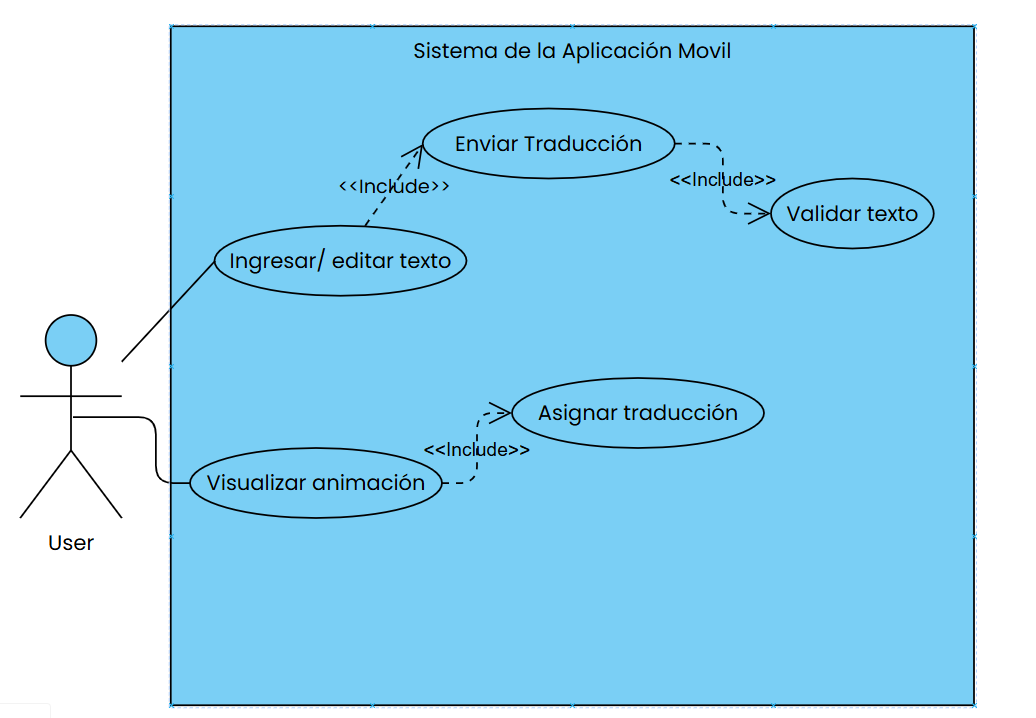
\includegraphics[width=0.6\textwidth]{Images/Cap 3/casodeuso1.png}
    \captionof{figure}{Diagrama de caso de uso 1}
\end{center}

\subsection{Mockups del sistema}
\begin{center}
    
\includegraphics[width=0.5\textwidth]{Images/Cap 3/Pantalla1.png}
    \captionof{figure}{Mockup de la pantalla de carga de la aplicación}
\end{center}

La primera pantalla que se muestra es la pantalla de carga de la aplicación, la cual muestra el mensaje "Espere por favor", junto con el ícono de un reloj para indicar que la app está cargando.

\begin{center}
    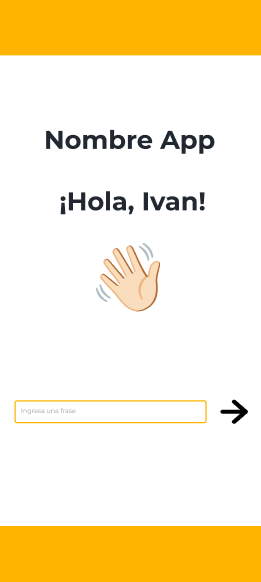
\includegraphics[width=0.5\textwidth]{Images/Cap 3/Pantalla2.png}
    \captionof{figure}{Mockup de la pantalla de ingreso de texto}
\end{center}

La seguda pantalla de la aplicación, la pantalla principal, es la pantalla para ingresar el texto. Se muestra el nombre de la app, un mensaje de bienvenida al usuario, un cuadro para ingresar el texto y un botón para acceder a la traducción.\\

Se debe ingresar texto en español dentro del cuadtro de entrada de texto, para que se realice todo el Procesamiento de Lenguaje Natural y mostrar la animación.

\begin{center}
    
\includegraphics[width=0.5\textwidth]{Images/Cap 3/Pantalla3.png}
    \captionof{figure}{Mockup de la pantalla la animación}
\end{center}

La tercera pantalla de la aplicación es la pantalla en donde se muestra la animación 3D de la traducción. Debajo del avatar 3D, se vuelve a mostrar el cuadro de entrada de texto para ingresar un nuevo mensaje.

\subsection{Identificación y evaluación de riesgos}
\subsubsection{Leyenda de probabilidad y efecto}
\textbf{Probabilidad:}
\begin{itemize}
	\item \textbf{Muy alta ($>$75\%):} Altamente probable que ocurra.
	\item \textbf{Alta (50-75\%):} Probable que ocurra en varias ocasiones durante el proyecto.
	\item \textbf{Moderada (25-50\%):} Existe una posibilidad razonable de que ocurra.
	\item \textbf{Baja (10-25\%):} Poco probable que ocurra, pero no imposible.
\end{itemize}

\textbf{Efecto (Impacto):}
\begin{itemize}
	\item \textbf{Catastrófico:} Afecta gravemente el éxito del proyecto, podría impedir la continuidad del mismo.
	\item \textbf{Serio:} Genera retrasos significativos o pérdida parcial de calidad en el desarrollo o resultados.
	\item \textbf{Tolerable:} Impacto menor, manejable sin afectar los objetivos generales del proyecto.
\end{itemize}


% ===== RIESGOS TÉCNICOS =====
\subsubsection{Riesgos técnicos}
Los riesgos técnicos están relacionados con las limitaciones de la tecnología utilizada, la precisión del modelo de traducción y la adaptación a las particularidades de la Lengua de Señas Mexicana (LSM).

\setlength{\tabcolsep}{4pt}
\renewcommand{\arraystretch}{1.2}

\begin{longtable}{|>{\centering\arraybackslash}p{0.8cm}|>{\raggedright\arraybackslash}p{3.5cm}|>{\raggedright\arraybackslash}p{5.1cm}|>{\raggedright\arraybackslash}p{5.1cm}|}
	\hline
	\textbf{ID} & \textbf{Riesgo específico} & \textbf{Probabilidad} & \textbf{Efecto} \\
	\hline
	T1 & Precisión limitada del modelo de traducción de español a LSM. & Alta (50-75\%) & Serio \\
	\hline
	T2 & Escasa disponibilidad de datasets de calidad para LSM. & Alta (50-75\%) & Serio \\
	\hline
	T3 & Desactualización tecnológica del modelo de IA frente a avances rápidos en el área. & Moderada (25-50\%) & Serio \\
	\hline
	T4 & Dificultad para manejar las variaciones regionales y culturales de LSM. & Media (25-50\%) & Catastrófico \\
	\hline
	T5 & Problemas de compatibilidad y funcionamiento multiplataforma. & Moderado (25-50\%) & Serio \\
	\hline
\caption{Resumen de riesgos técnicos} 
\label{tab:riesgos_tecnicos_resumen}
\end{longtable}

% ===== RIESGOS FINANCIEROS Y COMERCIALES =====
\subsubsection{Riesgos financieros y comerciales}
Estos riesgos afectan la viabilidad económica del proyecto y su posible escalamiento hacia una fase comercial.

\setlength{\tabcolsep}{4pt}
\renewcommand{\arraystretch}{1.2}

\begin{longtable}{|>{\centering\arraybackslash}p{0.8cm}|>{\raggedright\arraybackslash}p{3.5cm}|>{\raggedright\arraybackslash}p{5.1cm}|>{\raggedright\arraybackslash}p{5.1cm}|}
	\hline
	\textbf{ID} & \textbf{Riesgo específico} & \textbf{Probabilidad} & \textbf{Efecto} \\
	\hline
	F1 & Subestimación de los costos de producción y operación en una fase comercial. & Alta (50-75\%) & Catastrófico \\
	\hline
	F2 & Falta de modelos de negocio viables para monetizar la solución. & Moderada (25-50\%) & Serio \\
	\hline
	F3 & Dependencia de apoyos gubernamentales o financiamiento social para escalar el proyecto. & Media (25-50\%) & Serio \\
	\hline
	F4 & Competencia con otras soluciones similares con mayor madurez o presencia en el mercado. & Media (25-50\%) & Serio \\
	\hline
\caption{Resumen de riesgos financieros y comerciales} 
\label{tab:riesgos_financieros_resumen}
\end{longtable}

% ===== RIESGOS HUMANOS Y DE GESTIÓN =====
\subsubsection{Riesgos humanos y de gestión}
Estos riesgos se refieren a la disponibilidad, capacitación y coordinación del equipo, así como a la correcta gestión del proyecto.

\setlength{\tabcolsep}{4pt}
\renewcommand{\arraystretch}{1.2}

\begin{longtable}{|>{\centering\arraybackslash}p{0.8cm}|>{\raggedright\arraybackslash}p{3.5cm}|>{\raggedright\arraybackslash}p{5.1cm}|>{\raggedright\arraybackslash}p{5.1cm}|}
	\hline
	\textbf{ID} & \textbf{Riesgo específico} & \textbf{Probabilidad} & \textbf{Efecto} \\
	\hline
	H1 & Falta de experiencia del equipo en procesos de validación lingüística y cultural de LSM. & Alta (50-75\%) & Serio \\
	\hline
	H2 & Dependencia de colaboración externa para la validación de señas. & Media (25-50\%) & Serio \\
	\hline
	H3 & Desmotivación o alta rotación del equipo técnico. & Moderada (25-50\%) & Serio \\
	\hline
	H4 & Falta de claridad o definición adecuada de los requerimientos funcionales. & Alta (50-75\%) & Serio \\
	\hline
\caption{Resumen de riesgos humanos y de gestión} 
\label{tab:riesgos_humanoss_resumen}
\end{longtable}

% ===== RIESGOS ÉTICOS Y REGULATORIOS =====
\subsubsection{Riesgos éticos y regulatorios}
Riesgos asociados a las normativas, certificaciones y cuestiones éticas, especialmente por el tipo de aplicación y su uso potencial en contextos sensibles.

\setlength{\tabcolsep}{4pt}
\renewcommand{\arraystretch}{1.2}

\begin{longtable}{|>{\centering\arraybackslash}p{0.8cm}|>{\raggedright\arraybackslash}p{3.5cm}|>{\raggedright\arraybackslash}p{5.1cm}|>{\raggedright\arraybackslash}p{5.1cm}|}
	\hline
	\textbf{ID} & \textbf{Riesgo específico} & \textbf{Probabilidad} & \textbf{Efecto} \\
	\hline
	E1 & Interpretación incorrecta de mensajes sensibles (contexto médico, legal, etc.). & Baja (10-25\%) & Catastrófico \\
	\hline
	E2 & Ausencia de certificaciones o validaciones oficiales del modelo de traducción. & Moderada (25-50\%) & Serio \\
	\hline
	E3 & Uso no autorizado de bases de datos o glosarios protegidos. & Baja (10-25\%) & Catastrófico \\
	\hline
	E4 & Incumplimiento con normativas de accesibilidad digital o protección de datos. & Moderada (25-50\%) & Catastrófico \\
	\hline
\caption{Resumen de riesgos éticos y regulatorios} 
\label{tab:riesgos_eticos_resumen}
\end{longtable}

\newpage
\subsection{Planes de prevención y contingencia para riegos}

Esta sección describe las acciones preventivas y los planes de contingencia asociados a los riesgos identificados para el proyecto. La información se organiza por categoría de riesgo, facilitando la identificación y trazabilidad de las medidas frente a cada riesgo.

\subsubsection{Planes de prevención y contingencia para riesgos técnicos}

\setlength{\tabcolsep}{4pt}
\renewcommand{\arraystretch}{1.2}

\begin{longtable}{|>{\centering\arraybackslash}p{0.8cm}|>{\raggedright\arraybackslash}p{3.5cm}|>{\raggedright\arraybackslash}p{5.1cm}|>{\raggedright\arraybackslash}p{5.1cm}|}
	\hline
	\textbf{ID} & \textbf{Riesgo específico} & \textbf{Prevención} & \textbf{Plan de contingencia} \\
	\hline
	T1 & Precisión limitada del modelo de traducción de español a LSM. &
	\begin{itemize}
		\item Validar el modelo con expertos en LSM.
		\item Realizar pruebas piloto con retroalimentación continua.
		\item Incorporar técnicas de mejora continua en el entrenamiento.
	\end{itemize} &
	\begin{itemize}
		\item Ajustar el modelo mediante reentrenamiento con nuevos datos.
		\item Aplicar correcciones manuales temporales mientras se mejora la precisión.
		\item Evaluar modelos alternativos si el desempeño es insatisfactorio.
	\end{itemize} \\
	\hline
	T2 & Escasa disponibilidad de datasets de calidad para LSM. &
	\begin{itemize}
		\item Buscar colaboración con instituciones o expertos en LSM.
		\item Utilizar técnicas de data augmentation para ampliar los datos existentes.
	\end{itemize} &
	\begin{itemize}
		\item Integrar validaciones humanas adicionales para compensar la falta de datos.
		\item Ajustar el alcance del proyecto si los datos son insuficientes.
	\end{itemize} \\
	\hline
	T3 & Desactualización tecnológica del modelo de IA. &
	\begin{itemize}
		\item Mantener vigilancia tecnológica constante.
		\item Participar en foros y comunidades sobre IA y accesibilidad.
	\end{itemize} &
	\begin{itemize}
		\item Migrar a nuevas versiones o tecnologías según los avances detectados.
		\item Ajustar la arquitectura para facilitar futuras actualizaciones.
	\end{itemize} \\
	\hline
	T4 & Dificultad para manejar las variaciones regionales y culturales de LSM. &
	\begin{itemize}
		\item Buscar especialistas del área para el uso de región específica.
	\end{itemize} &
	\begin{itemize}
		\item Limitar el alcance del prototipo a ciertas regiones mientras se extiende la cobertura.
		\item Informar claramente las limitaciones del modelo a los usuarios.
	\end{itemize} \\
	\hline
	T5 & Problemas de compatibilidad y funcionamiento multiplataforma. &
	\begin{itemize}
		\item Desarrollar bajo estándares multiplataforma.
		\item Realizar pruebas en distintos dispositivos y navegadores.
	\end{itemize} &
	\begin{itemize}
		\item Aplicar correcciones específicas por plataforma detectada.
		\item Priorizar las plataformas con mayor demanda de usuarios.
	\end{itemize} \\
	\hline
	\caption{Planes de prevención y contingencia para riesgos técnicos} \label{tab:riesgos_tecnicos}
\end{longtable}


\newpage
% ========================
% Puedes continuar con las siguientes subsecciones:

\subsubsection{Planes de prevención y contingencia para riesgos financieros y comerciales}

\setlength{\tabcolsep}{4pt}
\renewcommand{\arraystretch}{1.2}

\begin{longtable}{|>{\centering\arraybackslash}p{0.8cm}|>{\raggedright\arraybackslash}p{3.5cm}|>{\raggedright\arraybackslash}p{5.1cm}|>{\raggedright\arraybackslash}p{5.1cm}|}
	\hline
	\textbf{ID} & \textbf{Riesgo específico} & \textbf{Prevención} & \textbf{Plan de contingencia} \\
	\hline
	F1 & Subestimación de los costos de producción y operación en una fase comercial. &
	\begin{itemize}
		\item Elaborar un análisis financiero detallado con escenarios conservadores.
		\item Incluir márgenes de contingencia en la planificación de costos.
	\end{itemize} &
	\begin{itemize}
		\item Reevaluar los costos y ajustar el modelo de negocio.
		\item Buscar financiamiento adicional o ajustar el alcance del proyecto.
	\end{itemize} \\
	\hline
	F2 & Falta de modelos de negocio viables para monetizar la solución. &
	\begin{itemize}
		\item Diseñar y evaluar diferentes modelos de negocio desde la fase temprana.
		\item Consultar expertos en comercialización y accesibilidad.
	\end{itemize} &
	\begin{itemize}
		\item Ajustar la estrategia hacia modelos freemium, licencias o apoyos institucionales.
		\item Explorar alianzas con organizaciones del sector social o educativo.
	\end{itemize} \\
	\hline
	F3 & Dependencia de apoyos gubernamentales o financiamiento social para escalar el proyecto. &
	\begin{itemize}
		\item Diversificar las posibles fuentes de financiamiento (fondos privados, crowdfunding).
		\item Preparar la documentación requerida para aplicar a diferentes programas.
	\end{itemize} &
	\begin{itemize}
		\item Redimensionar el proyecto a una escala mínima viable si no se obtienen los fondos esperados.
		\item Buscar inversionistas privados o aliados estratégicos.
	\end{itemize} \\
	\hline
	F4 & Competencia con otras soluciones similares con mayor madurez o presencia en el mercado. &
	\begin{itemize}
		\item Realizar un monitoreo constante del mercado y de las soluciones existentes.
		\item Diferenciar la propuesta de valor en facilidad de uso, precio o calidad.
	\end{itemize} &
	\begin{itemize}
		\item Ajustar el enfoque del producto según las necesidades no cubiertas por la competencia.
		\item Enfocar el desarrollo en nichos específicos o sectores desatendidos.
	\end{itemize} \\
	\hline
	\caption{Planes de prevención y contingencia para riesgos financieros y comerciales}
	 \label{tab:riesgos_financieros}
\end{longtable}

\newpage

\subsubsection{Planes de prevención y contingencia para riesgos humanos y de gestión}

\setlength{\tabcolsep}{4pt}
\renewcommand{\arraystretch}{1.2}

\begin{longtable}{|>{\centering\arraybackslash}p{0.8cm}|>{\raggedright\arraybackslash}p{3.5cm}|>{\raggedright\arraybackslash}p{5.1cm}|>{\raggedright\arraybackslash}p{5.1cm}|}
	\hline
	\textbf{ID} & \textbf{Riesgo específico} & \textbf{Prevención} & \textbf{Plan de contingencia} \\
	\hline
	H1 & Falta de experiencia del equipo en validación lingüística y cultural de LSM. &
	\begin{itemize}
		\item Incluir asesoría de expertos en LSM durante el desarrollo.
		\item Capacitar al equipo en aspectos básicos de la cultura y lengua de señas.
	\end{itemize} &
	\begin{itemize}
		\item Contratar o colaborar con intérpretes certificados para cubrir las áreas necesarias.
		\item Ajustar las pruebas de validación incorporando especialistas externos.
	\end{itemize} \\
	\hline
	H2 & Dependencia de colaboración externa para la validación de señas. &
	\begin{itemize}
		\item Establecer acuerdos formales con colaboradores e intérpretes desde el inicio.
		\item Definir tiempos y compromisos claros de participación.
	\end{itemize} &
	\begin{itemize}
		\item Buscar reemplazos o alianzas adicionales si algún colaborador no cumple lo acordado.
		\item Ajustar el cronograma para incluir tiempo adicional si se presentan retrasos.
	\end{itemize} \\
	\hline
	H3 & Desmotivación o alta rotación del equipo técnico. &
	\begin{itemize}
		\item Fomentar un ambiente laboral positivo y flexible.
		\item Ofrecer oportunidades de aprendizaje y desarrollo profesional.
	\end{itemize} &
	\begin{itemize}
		\item Redistribuir funciones y roles de manera temporal.
		\item Contratar personal de refuerzo o apoyo externo si es necesario.
	\end{itemize} \\
	\hline
	H4 & Falta de claridad o definición adecuada de los requerimientos funcionales. &
	\begin{itemize}
		\item Documentar los requisitos de manera detallada y validarlos con los stakeholders.
		\item Realizar sesiones de revisión y ajuste de requisitos de forma periódica.
	\end{itemize} &
	\begin{itemize}
		\item Detener las tareas críticas hasta tener claridad total sobre los requisitos.
		\item Reorganizar el backlog y ajustar las prioridades si es necesario.
	\end{itemize} \\
	\hline
	\caption{Planes de prevención y contingencia para riesgos humanos y de gestión} 
	\label{tab:riesgos_humanos}
\end{longtable}

\subsubsection{Planes de prevención y contingencia para riesgos éticos y regulatorios}

\setlength{\tabcolsep}{4pt}
\renewcommand{\arraystretch}{1.2}

\begin{longtable}{|>{\centering\arraybackslash}p{0.8cm}|>{\raggedright\arraybackslash}p{3.5cm}|>{\raggedright\arraybackslash}p{5.1cm}|>{\raggedright\arraybackslash}p{5.1cm}|}
	\hline
	\textbf{ID} & \textbf{Riesgo específico} & \textbf{Prevención} & \textbf{Plan de contingencia} \\
	\hline
	E1 & Interpretación incorrecta de mensajes sensibles (contexto médico, legal, etc.). &
	\begin{itemize}
		\item Definir claramente los contextos de uso permitidos del sistema.
		\item Incluir advertencias sobre los límites del modelo en el uso de la aplicación.
	\end{itemize} &
	\begin{itemize}
		\item Limitar temporalmente las funcionalidades en contextos de alto riesgo.
		\item Incorporar revisiones humanas en casos sensibles o críticos.
	\end{itemize} \\
	\hline
	E2 & Ausencia de certificaciones o validaciones oficiales del modelo de traducción. &
	\begin{itemize}
		\item Investigar los procesos de certificación existentes y planear la obtención de las acreditaciones.
		\item Involucrar expertos en accesibilidad y traducción en el proceso de validación.
	\end{itemize} &
	\begin{itemize}
		\item Buscar asesoría externa para cumplir los requisitos regulatorios si se identifican brechas.
		\item Ajustar la fase comercial hasta obtener las validaciones requeridas.
	\end{itemize} \\
	\hline
	E3 & Uso no autorizado de conjunto de datos o glosarios protegidos. &
	\begin{itemize}
		\item Verificar licencias de uso de todos los recursos desde la etapa de diseño.
		\item Priorizar el uso de datos open-source o desarrollados internamente.
	\end{itemize} &
	\begin{itemize}
		\item Sustituir inmediatamente los recursos cuestionados por alternativas con licencias válidas.
		\item Consultar asesoría legal para resolver posibles conflictos de derechos de autor.
	\end{itemize} \\
	\hline
	E4 & Incumplimiento con normativas de accesibilidad digital o protección de datos. &
	\begin{itemize}
		\item Asegurar el cumplimiento de la norma ISO 9241-210:2019 y Heurísticas de Jakob Nielsen.
		\item Consultar especialistas en regulación y accesibilidad.
	\end{itemize} &
	\begin{itemize}
		\item Corregir los puntos de incumplimiento detectados antes del lanzamiento comercial.
		\item Documentar y comunicar las acciones correctivas a los usuarios y autoridades si es necesario.
	\end{itemize} \\
	\hline
\caption{Planes de prevención y contingencia para riesgos éticos y regulatorios} \label{tab:riesgos_eticos} \\
\end{longtable}


\section{Selección de los datos}
\subsection{Recolección de datos}

\section{Preparación de los datos}

\chapter{Conclusiones}
En la primera etapa desarrollada del Trabajo Terminal, se establecen las bases teóricas y técnicas necesarias para el desarrollo de una solución tecnológica inclusiva orientada a mejorar la comunicación entre personas oyentes y personas con discapacidad auditiva. A partir del análisis de la motivación, la problemática y los objetivos del proyecto, se delimita un enfoque centrado en la accesibilidad lingüística a través de la Lengua de Señas Mexicana (LSM).\\

La revisión del estado del arte y la construcción del marco teórico permiten contextualizar el proyecto dentro del ámbito del procesamiento de lenguaje natural y la representación visual mediante modelado 3D, evidenciando que, si bien existen herramientas similares a nivel internacional, estas no abordan de manera específica las características lingüísticas, culturales y gramaticales de la LSM. Asimismo, el análisis del proceso de comunicación y el estudio profundo de los elementos lingüísticos de esta lengua (como su estructura espacial, dactilología, fonología y gramática) revela los desafíos técnicos de su implementación digital y la necesidad de soluciones adaptadas al contexto mexicano.


\chapter{Referencias}


\chapter{Trabajo relacionado}

\chapter{Desarrollo}

\chapter{Experimentos}

\chapter{Conclusiones y trabajo futuro}

\appendix
\chapter*{Anexos}
\addcontentsline{toc}{chapter}{Anexos}

\chapter{Cuestionario aplicado}
